\chapter{Probability}

\section{Frequentists vs. Bayesians}
what is probability? \textbf{frequentist} interpretation vs. \textbf{Bayesian} interpretation.

One big advantage of the Bayesian interpretation is that it can be used to model our uncertainty about events that do not have long term frequencies.

Therefore most machine learning books adopt the Bayesian interpretation. Fortunately, the basic rules of probability theory are the same, no matter which interpretation is adopted.


\section{A brief review of probability theory}


\subsection{Basic concepts}
We denote a random event by defining a \textbf{random variable} $X$.

\textbf{Descrete random variable}: $X$ can take on any value from a finite or countably infinite set.

\textbf{Continuous random variable}: the value of $X$ is real-valued.


\subsubsection{CDF}

\begin{equation}
F(x) \triangleq P(X \leq x)=\begin{cases}
\sum_{u \leq x}p(u), & \text{descrete random variable}\\
\int_{-\infty}^{x} f(u)du, & \text{continuous random variable}\\
\end{cases}
\end{equation}


\subsubsection{PMF and PDF}
For descrete random variable, We denote the probability of the event that $X=x$ by $P(X=x)$, or just $p(x)$ for short. Here $p(x)$ is called a \textbf{probability mass function} or \textbf{PMF}.A probability mass function is a function that gives the probability that a discrete random variable is exactly equal to some value\footnote{\url{http://en.wikipedia.org/wiki/Probability_mass_function}}. This satisfies the properties $0 \leq p(x) \leq 1$ and $\sum_{x \in \mathcal{X}} p(x)=1$.

For continuous variable, in the equation $F(x)=\int_{-\infty}^{x} f(u)du$, the function $f(x)$ is called a \textbf{probability density function} or \textbf{PDF}. A probability density function is a function that describes the relative likelihood for this random variable to take on a given value\footnote{\url{http://en.wikipedia.org/wiki/Probability_density_function}}.This satisfies the properties $f(x) \geq 0$ and $\int_{-\infty}^{\infty} f(x)dx=1$.


\subsection{Mutivariate random variables}


\subsubsection{Joint CDF}
We denote joint CDF by $F(x,y) \triangleq P(X \leq x \cap Y \leq y)=P(X \leq x , Y \leq y)$.

\begin{equation}
F(x,y) \triangleq P(X \leq x, Y \leq y)=\begin{cases}
\sum_{u \leq x, v \leq y}p(u,v), & \text{descrete}\\
\int_{-\infty}^{x}\int_{-\infty}^{y} f(u,v)dudv, & \text{continuous}\\
\end{cases}
\end{equation}

\textbf{product rule}:
\begin{equation}
p(X,Y)=P(X|Y)P(Y)
\end{equation}

\textbf{Chain rule}:
\begin{equation}
p(X_{1:N})=p(X_1)p(X_2|X_1)p(X_3|X_2,X_1)...p(X_N|X_{1:N-1})
\end{equation}


\subsubsection{Marginal distribution}
\textbf{Marginal CDF}:
\begin{equation}
\begin{cases}
F_X(x) \triangleq F(x,+\infty)=\begin{cases}
\sum_{x_i \leq x}P(X=x_i)=\sum_{x_i \leq x}\sum_{j=1}^{+\infty}P(X=x_i,Y=y_j), & \text{descrete}\\
\int_{-\infty}^{x}f_X(u)du=\int_{-\infty}^{x}\int_{-\infty}^{+\infty} f(u,v)dudv, & \text{continuous}\\
\end{cases}\\
F_Y(y) \triangleq F(+\infty,y)=\begin{cases}
\sum_{y_j \leq y}p(Y=y_j)=\sum_{i=1}^{+\infty}\sum_{y_j \leq y}P(X=x_i,Y=y_j), & \text{descrete}\\
\int_{-\infty}^{y}f_Y(v)dv=\int_{-\infty}^{+\infty}\int_{-\infty}^{y} f(u,v)dudv, & \text{continuous}\\
\end{cases}\\
\end{cases}
\end{equation}

\textbf{Marginal PMF or PDF}:
\begin{equation}
\begin{cases}
\begin{cases}
P(X=x_i)=\sum_{j=1}^{+\infty}P(X=x_i,Y=y_j), & \text{descrete}\\
f_X(x)=\int_{-\infty}^{+\infty} f(x,y)dy, & \text{continuous}\\
\end{cases}\\
\begin{cases}
p(Y=y_j)=\sum_{i=1}^{+\infty}P(X=x_i,Y=y_j), & \text{descrete}\\
f_Y(y)=\int_{-\infty}^{+\infty} f(x,y)dx, & \text{continuous}\\
\end{cases}\\
\end{cases}
\end{equation}


\subsubsection{Conditional distribution}
\textbf{Conditional PMF}:
\begin{equation}
p(X=x_i|Y=y_j)=\dfrac{p(X=x_i,Y=y_j)}{p(Y=y_j)} \text{ if } p(Y)>0
\end{equation}
The pmf $p(X|Y)$ is called \textbf{conditional probability}.

\textbf{Conditional PDF}:
\begin{equation}
f_{X|Y}(x|y)=\dfrac{f(x,y)}{f_Y(y)}
\end{equation}

\subsection{Bayes rule}
\begin{equation}
p(Y=y|X=x)=\dfrac{p(X=x,Y=y)}{p(X=x)}=\dfrac{p(X=x|Y=y)p(Y=y)}{\sum_{y'}p(X=x|Y=y')p(Y=y')}
\end{equation}

\subsubsection{Example: Generative classifiers}
\begin{equation}
p(y=c|X,\vec{\theta})=\dfrac{p(X|y=c,\vec{\theta})p(y=c|\vec{\theta})}{\sum_{c'}p(X|y=c',\vec{\theta})p(y=c'|\vec{\theta})}
\end{equation}

This is called a \textbf{generative classifier}, since it specifies how to generate the data using the class conditional density $p(x|y=c)$ and the class prior $p(y = c)$. An alternative approach is to directly fit the class posterior, $p(y=c|x)$ ;this is known as a \textbf{discriminative classifier}. 

\subsection{Independence and conditional independence}
We say $X$ and $Y$ are unconditionally independent or marginally independent, denoted $X \perp Y$, if we can represent the joint as the product of the two marginals, i.e.,
\begin{equation}
X \perp Y=P(X,Y)=P(X)P(Y)
\end{equation}

We say $X$ and $Y$ are conditionally independent(CI) given $Z$ if the conditional joint can be written as a product of conditional marginals:
\begin{equation}
X \perp Y|Z=P(X,Y|Z)=P(X|Z)P(Y|Z)
\end{equation}

\subsection{Quantiles}
Since the cdf $F$ is a monotonically increasing function, it has an inverse; let us denote this by $F^{-1}$. If $F$ is the cdf of $X$ , then $F^{-1}(\alpha)$ is the value of $x_{\alpha}$ such that $P(X \leq x_{\alpha})=\alpha$; this is called the $\alpha$ quantile of $F$. The value $F^{-1}(0.5)$ is the \textbf{median} of the distribution, with half of the probability mass on the left, and half on the right. The values $F^{-1}(0.25)$ and $F^{−1}(0.75)$are the lower and upper \textbf{quartiles}.

\subsection{Mean and variance}
The most familiar property of a distribution is its \textbf{mean},or \textbf{expected value}, denoted by $\mu$. For discrete rv’s, it is defined as $\mathbb{E}[X] \triangleq \sum_{x \in \mathcal{X}}xp(x)$, and for continuous rv’s, it is defined as $\mathbb{E}[X] \triangleq \int_{\mathcal{X}}xp(x)dx$. If this integral is not finite, the mean is not defined (we will see some examples of this later). 

The \textbf{variance} is a measure of the “spread” of a distribution, denoted by $\sigma^2$. This is defined as follows:
\begin{eqnarray}
var[X]&=&\mathbb{E}[(X-\mu)^2]=\int{(x-\mu)^2p(x)dx}\\
      &=&\int{x^2p(x)dx}\int{{\mu}^2p(x)dx}-2\mu\int{xp(x)dx}=\mathbb{E}[X^2]-{\mu}^2
\end{eqnarray}

from which we derive the useful result
\begin{equation}
\mathbb{E}[X^2]=\sigma^2+{\mu}^2
\end{equation}

The \textbf{standard deviation} is defined as
\begin{equation}
std[X] \triangleq =\sqrt{var[X]}
\end{equation}

This is useful since it has the same units as $X$ itself.

\section{Some common discrete distributions}
In this section, we review some commonly used parametric distributions defined on discrete state spaces, both finite and countably infinite.


\subsection{The binomial and Bernoulli distributions}


\subsection{The multinomial and multinoulli distributions}


\subsection{The Poisson distribution}


\subsection{The empirical distribution}


\section{Some common continuous distributions}
In this section we present some commonly used univariate (one-dimensional) continuous probability distributions.


\subsection{Gaussian (normal) distribution}


\subsection{Degenerate pdf}


\subsection{The Laplace distribution}


\subsection{The gamma distribution}


\subsection{The beta distribution}


\subsection{Pareto distribution}


\section{Information theory}

\subsection{Entropy}
\label{sec:Entropy}
The entropy of a random variable $X$ with distribution $p$, denoted by $\mathbb{H}(X)$ or sometimes $\mathbb{H}(p)$, is a measure of its uncertainty. In particular, for a discrete variable with $K$ states, it is defined by
\begin{equation}
\mathbb{H}(X) \triangleq -\sum\limits_{k=1}^{K}{p(X=k)\log_2p(X=k)}
\end{equation}

Usually we use log base 2, in which case the units are called \textbf{bits}(short for binary digits). If we use log base $e$ , the units are called \textbf{nats}. 

The discrete distribution with maximum entropy is the uniform distribution (see Section XXX for a proof). Hence for a K-ary random variable, the entropy is maximized if $p(x = k)=1/K$; in this case, $\mathbb{H}(X)=\log_2K$. 

Conversely, the distribution with minimum entropy (which is zero) is any \textbf{delta-function} that puts all its mass on one state. Such a distribution has no uncertainty.


\subsection{KL divergence}
One way to measure the dissimilarity of two probability distributions, $p$ and $q$ , is known as the \textbf{Kullback-Leibler divergence}(\textbf{KL divergence})or \textbf{relative entropy}. This is defined as follows:
\begin{equation}
\mathbb{KL}(P||Q) \triangleq 
\sum\limits_{x}{p(x)\log_2\dfrac{p(x)}{q(x)}}
\end{equation}
where the sum gets replaced by an integral for pdfs\footnote{The KL divergence is not a distance, since it is asymmetric. One symmetric version of the KL divergence is the \textbf{Jensen-Shannon divergence}, defined as $JS(p_1,p_2)=0.5\mathbb{KL}(p_1||q)+0.5\mathbb{KL}(p_2||q)$,where $q=0.5p_1+0.5p_2$}. The KL divergence is only defined if P and Q both sum to 1 and if $q(x)=0$ implies $p(x)=0$ for all $x$(absolute continuity). If the quantity  $0\ln0$ appears in the formula, it is interpreted as zero because $\lim\limits_{x \to 0}x\ln x$. We can rewrite this as
\begin{equation}
\mathbb{KL}(p||q) \triangleq \sum\limits_{x}{p(x)\log_2p(x)}-\sum\limits_{k=1}^{K}{p(x)\log_2q(x)}=\mathbb{H}(p)-\mathbb{H}(p,q)
\end{equation}
where $\mathbb{H}(p,q)$ is called the \textbf{cross entropy},
\begin{equation}
\mathbb{H}(p,q)=\sum\limits_{x}{p(x)\log_2q(x)}
\end{equation}

One can show (Cover and Thomas 2006) that the cross entropy is the average number of bits needed to encode data coming from a source with distribution $p$ when we use model $q$ to define our codebook. Hence the “regular” entropy $\mathbb{H}(p)=\mathbb{H}(p,p)$, defined in section \S \ref{sec:Entropy},is the expected number of bits if we use the true model, so the KL divergence is the diference between these. In other words, the KL divergence is the average number of \emph{extra} bits needed to encode the data, due to the fact that we used distribution $q$ to encode the data instead of the true distribution $p$.

The “extra number of bits” interpretation should make it clear that $\mathbb{KL}(p||q) \geq 0$, and that the KL is only equal to zero if $q = p$. We now give a proof of this important result.

\begin{theorem}
(\textbf{Information inequality}) $\mathbb{KL}(p||q) \geq 0 \text{ with equality iff } p=q$.
\end{theorem}

One important consequence of this result is that \emph{the discrete distribution with the maximum
entropy is the uniform distribution}.


\subsection{Mutual information}
\begin{definition}
\textbf{Mutual information} or \textbf{MI}, is defined as follows:
\begin{equation}
\mathbb{I}(X;Y) \triangleq \mathbb{KL}(P(X,Y)||P(X)P(X))=\sum\limits_x\sum\limits_yp(x,y)\log\dfrac{p(x,y)}{p(x)p(y)}
\end{equation}
We have $\mathbb{I}(X;Y) \geq 0$ with equality if $P(X,Y)=P(X)P(Y)$. That is, the MI is zero if the variables are independent.
\end{definition}

To gain insight into the meaning of MI, it helps to re-express it in terms of joint and conditional entropies. One can show that the above expression is equivalent to the following:
\begin{eqnarray}
\mathbb{I}(X;Y)&=&\mathbb{H}(X)-\mathbb{H}(X|Y)\\
               &=&\mathbb{H}(Y)-\mathbb{H}(Y|X)\\
               &=&\mathbb{H}(X)+\mathbb{H}(Y)-\mathbb{H}(X,Y)\\
               &=&\mathbb{H}(X,Y)-\mathbb{H}(X|Y)-\mathbb{H}(Y|X)
\end{eqnarray}
where $\mathbb{H}(X)$ and $\mathbb{H}(Y)$ are the \textbf{marginal entropies}, $\mathbb{H}(X|Y)$ and $\mathbb{H}(Y|X)$ are the \textbf{conditional entropies}, and $\mathbb{H}(X,Y)$ is the \textbf{joint entropy} of $X$ and $Y$, see Fig. ~\ref{fig:mi}\footnote{\url{http://en.wikipedia.org/wiki/Mutual_information}}.

\begin{figure}[hbtp]
\centering
    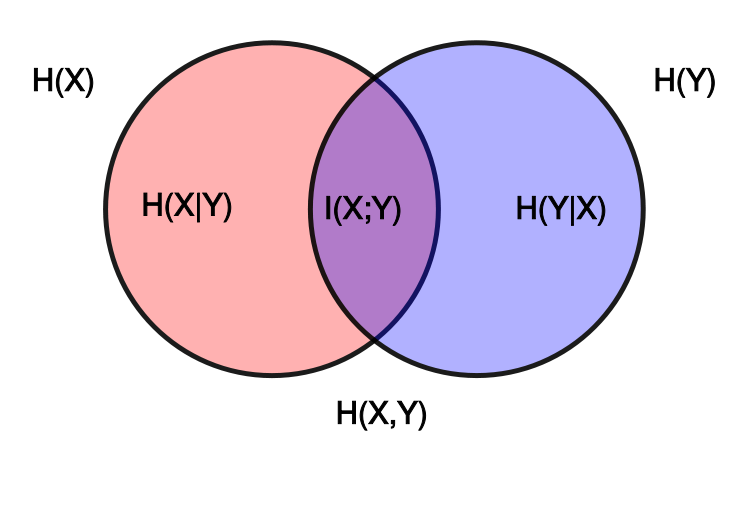
\includegraphics[scale=.25]{figures/mutual-information.png}
\caption{Individual $\mathbb{H}(X),\mathbb{H}(Y)$, joint $\mathbb{H}(X,Y)$, and conditional entropies for a pair of correlated subsystems $X,Y$ with mutual information $\mathbb{I}(X;Y)$.}
\label{fig:mi} 
\end{figure}

Intuitively, we can interpret the MI between $X$ and $Y$ as the reduction in uncertainty about $X$ after observing $Y$, or, by symmetry, the reduction in uncertainty about $Y$ after observing $X$.

A quantity which is closely related to MI is the \textbf{pointwise mutual information} or \textbf{PMI}. For two events (not random variables) $x$ and $y$, this is defined as
\begin{equation}
PMI(x,y) \triangleq \log\dfrac{p(x,y)}{p(x)p(y)}=\log\dfrac{p(x|y)}{p(x)}=\log\dfrac{p(y|x)}{p(y)}
\end{equation}

This measures the discrepancy between these events occuring together compared to what would be expected by chance. Clearly the MI of $X$ and $Y$ is just the expected value of the PMI. Interestingly, we can rewrite the PMI as follows:
\begin{equation}
PMI(x,y)=\log\dfrac{p(x|y)}{p(x)}=\log\dfrac{p(y|x)}{p(y)}
\end{equation}

This is the amount we learn from updating the prior $p(x)$ into the posterior $p(x|y)$ , or equivalently, updating the prior $p(y)$ into the posterior $p(y |x)$ .